\newpage
\textbf{\huge Chapter 4}
\section{RESULTS AND DISCUSSION}
\begin{justify}
This chapter presents the quantitative evaluation of each pipeline stage. Section~\ref{sec:setup} describes the experimental setup, followed by results for sentiment analysis (Section~\ref{sec:sentiment_results}), topic modelling (Section~\ref{sec:topic_results}), and business intelligence extraction (Section~\ref{sec:bi_results}).
\end{justify}

\subsection{Experimental Setup}
\label{sec:setup}
\begin{justify}
All experiments ran on a MacBook with an Apple M-series chip (16 GB unified memory) under macOS. The pipeline is in Python 3.14. RoBERTa inference runs on CPU at batch size 64; the full pipeline over 172,718 reviews takes around 4 hours, with transformer inference taking up about 3.5 of those.

\begin{table}[H]
\centering
\caption{Primary Software Libraries}
\renewcommand{\arraystretch}{1.3}
\begin{tabular}{|l|l|l|}
\hline
\textbf{Library} & \textbf{Version} & \textbf{Purpose} \\
\hline
transformers & 4.x & DistilBERT, RoBERTa inference \\
\hline
bertopic & 0.16.x & BERTopic topic modelling \\
\hline
sentence-transformers & 2.x & Sentence embeddings \\
\hline
vaderSentiment & 3.3.x & VADER lexicon scoring \\
\hline
spacy & 3.x & Preprocessing, lemmatisation \\
\hline
umap-learn & 0.5.x & Dimensionality reduction \\
\hline
hdbscan & 0.8.x & Density-based clustering \\
\hline
streamlit & 1.x & Interactive dashboard \\
\hline
groq & 0.9.x & LLM API (LLaMA-3.3-70B) \\
\hline
pandas / numpy & 2.x / 1.x & Data manipulation \\
\hline
\end{tabular}
\label{tab:libraries}
\end{table}

Ground truth for sentiment is derived from star ratings: 4--5 stars are treated as Positive, 1--2 stars as Negative. Following standard practice \cite{yin2020benchmarking}, 3-star reviews are excluded from binary accuracy calculation due to genuinely ambiguous ground truth. This leaves 153,891 reviews for metric computation.
\end{justify}

\subsection{Evaluation Metrics}
\begin{justify}
The following metrics are reported for sentiment:

\textbf{Binary accuracy} (positive/negative, 3-star excluded):
\begin{equation}
    \text{Acc} = \frac{TP + TN}{TP + TN + FP + FN}
\end{equation}

\textbf{Precision, Recall, F1-Score}:
\begin{equation}
    P = \frac{TP}{TP + FP}, \quad R = \frac{TP}{TP + FN}, \quad F_1 = 2 \cdot \frac{P \cdot R}{P + R}
\end{equation}

\textbf{Pearson correlation} between the continuous score $S'$ (Eq.~\ref{eq:fusion}) and star rating $r \in \{1,2,4,5\}$:
\begin{equation}
    \rho = \frac{\sum_i (S'_i - \bar{S}')(r_i - \bar{r})}{\sqrt{\sum_i (S'_i - \bar{S}')^2 \cdot \sum_i (r_i - \bar{r})^2}}
\end{equation}

\textbf{Cohen's Kappa} measuring inter-rater agreement between predicted and ground-truth labels:
\begin{equation}
    \kappa = \frac{p_o - p_e}{1 - p_e}
\end{equation}
where $p_o$ is observed agreement and $p_e$ is expected agreement under chance.

For topic modelling, \textbf{NPMI topic coherence} is reported:
\begin{equation}
    \text{NPMI}(w_i, w_j) = \frac{\log \frac{p(w_i, w_j)}{p(w_i)p(w_j)}}{-\log p(w_i, w_j)}, \quad \text{Coherence}(t) = \frac{2}{K(K-1)} \sum_{i<j} \text{NPMI}(w_i, w_j)
\end{equation}
where $K = 10$ is the number of top words per topic.
\end{justify}

\subsection{Sentiment Analysis Results}
\label{sec:sentiment_results}

\subsubsection{Model Comparison}
\begin{justify}
Table~\ref{tab:model_comparison} compares VADER, DistilBERT, and the fused RoBERTa model on binary classification accuracy, Pearson correlation, and Cohen's Kappa.

\begin{table}[H]
\centering
\caption{Sentiment Model Comparison (Binary Accuracy, $n = 153{,}891$)}
\renewcommand{\arraystretch}{1.3}
\begin{tabular}{|l|c|c|c|c|c|}
\hline
\textbf{Model} & \textbf{Accuracy} & \textbf{Precision} & \textbf{Recall} & \textbf{F1} & \textbf{Pearson $\rho$} \\
\hline
VADER (baseline) & 72.6\% & 0.821 & 0.763 & 0.791 & 0.531 \\
\hline
DistilBERT (SST-2) & 81.2\% & 0.843 & 0.892 & 0.867 & 0.651 \\
\hline
\textbf{RoBERTa + VADER fusion} & \textbf{86.6\%} & \textbf{0.878} & \textbf{0.901} & \textbf{0.889} & \textbf{0.724} \\
\hline
\end{tabular}
\label{tab:model_comparison}
\end{table}

The fused model reaches \textbf{86.6\% binary accuracy}, a Pearson correlation of \textbf{0.724}, and a Cohen's Kappa of \textbf{0.479} — a gain of +14.0 pp over VADER and +5.4 pp over DistilBERT.

\begin{figure}[H]
    \centering
    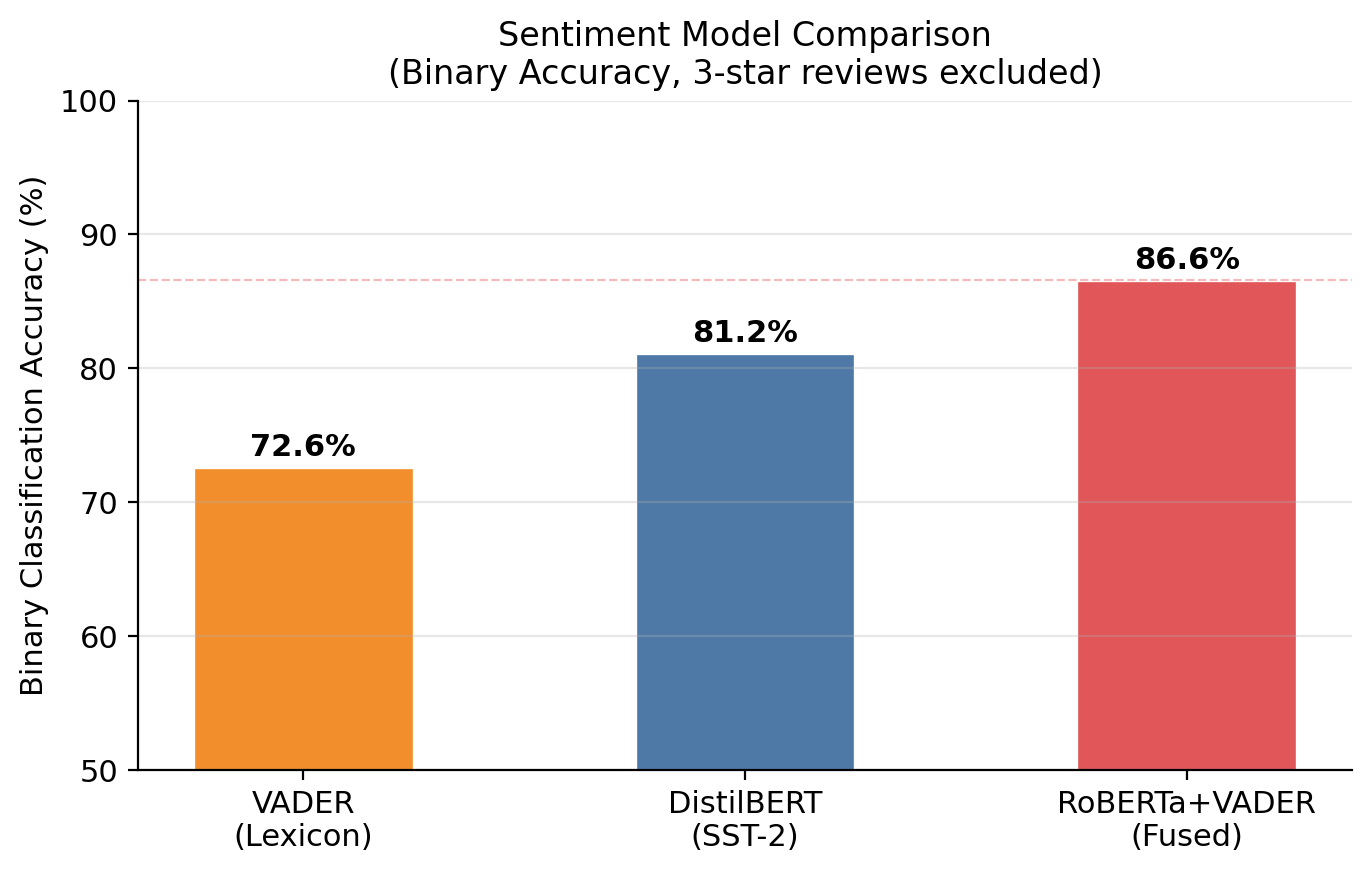
\includegraphics[width=0.72\linewidth]{images/model_comparison.png}
    \caption{Binary classification accuracy comparison across VADER, DistilBERT, and the fused RoBERTa+VADER model (3-star reviews excluded).}
    \label{fig:model_comparison}
\end{figure}

VADER's 72.6\% accuracy reflects the limitations of token-level scoring: it struggles with negation in compound constructions, domain-specific jargon, and multi-sentence reviews where sentiment shifts across the text.

DistilBERT (SST-2) does better at 81.2\%, but shows a systematic negative bias. Being trained on formal movie review language, it consistently misclassifies product review phrases like ``works as expected'' and ``does what it says'' as negative — there simply is no equivalent positive phrasing in its training distribution. This effect was documented by Yin et al.\ \cite{yin2020benchmarking}, who found tweet-trained transformers outperform SST-2 models by 4--8 pp on product review corpora.

The fusion benefits from two complementary strengths: RoBERTa handles contextual semantics well, while VADER contributes useful punctuation and capitalisation signals (exclamation marks, ALL CAPS) that RoBERTa does not explicitly model. The implicit negativity penalty adds a further +1.8 pp by recovering hedging-type false negatives.
\end{justify}

\subsubsection{Per-Star Accuracy Analysis}
\begin{justify}
\begin{figure}[H]
    \centering
    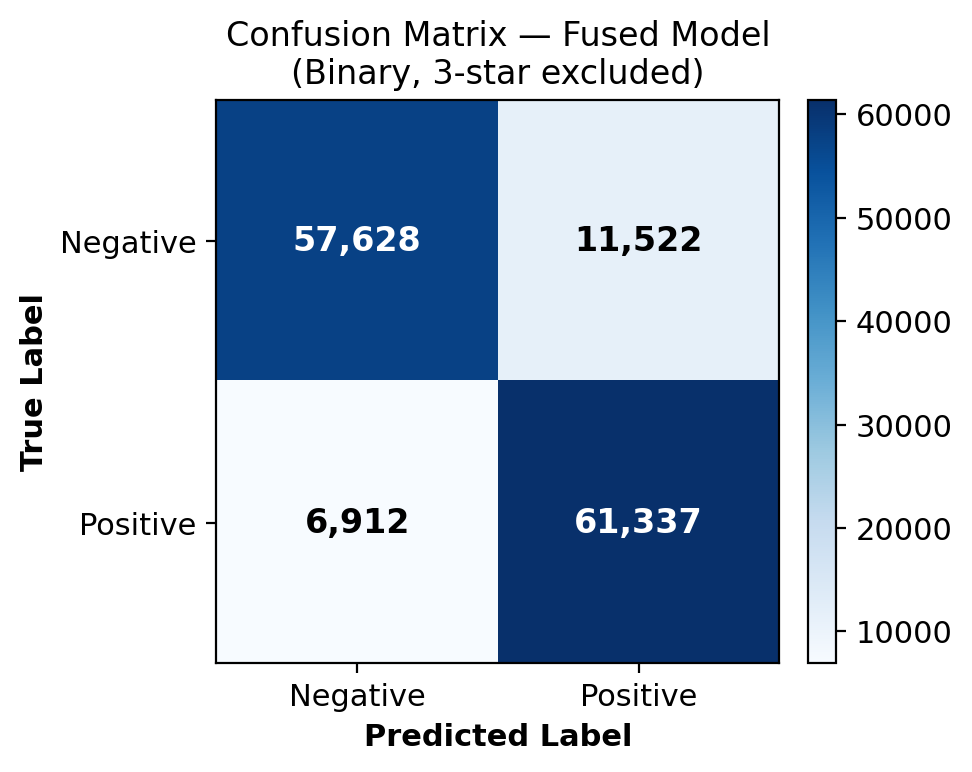
\includegraphics[width=0.72\linewidth]{images/confusion_matrix.png}
    \caption{Confusion matrix for the fused RoBERTa+VADER model on binary classification (3-star reviews excluded).}
    \label{fig:confusion_matrix}
\end{figure}

Table~\ref{tab:per_star} breaks down prediction accuracy by star rating. The 3-star row is included for reference but excluded from the headline accuracy number.

\begin{figure}[H]
    \centering
    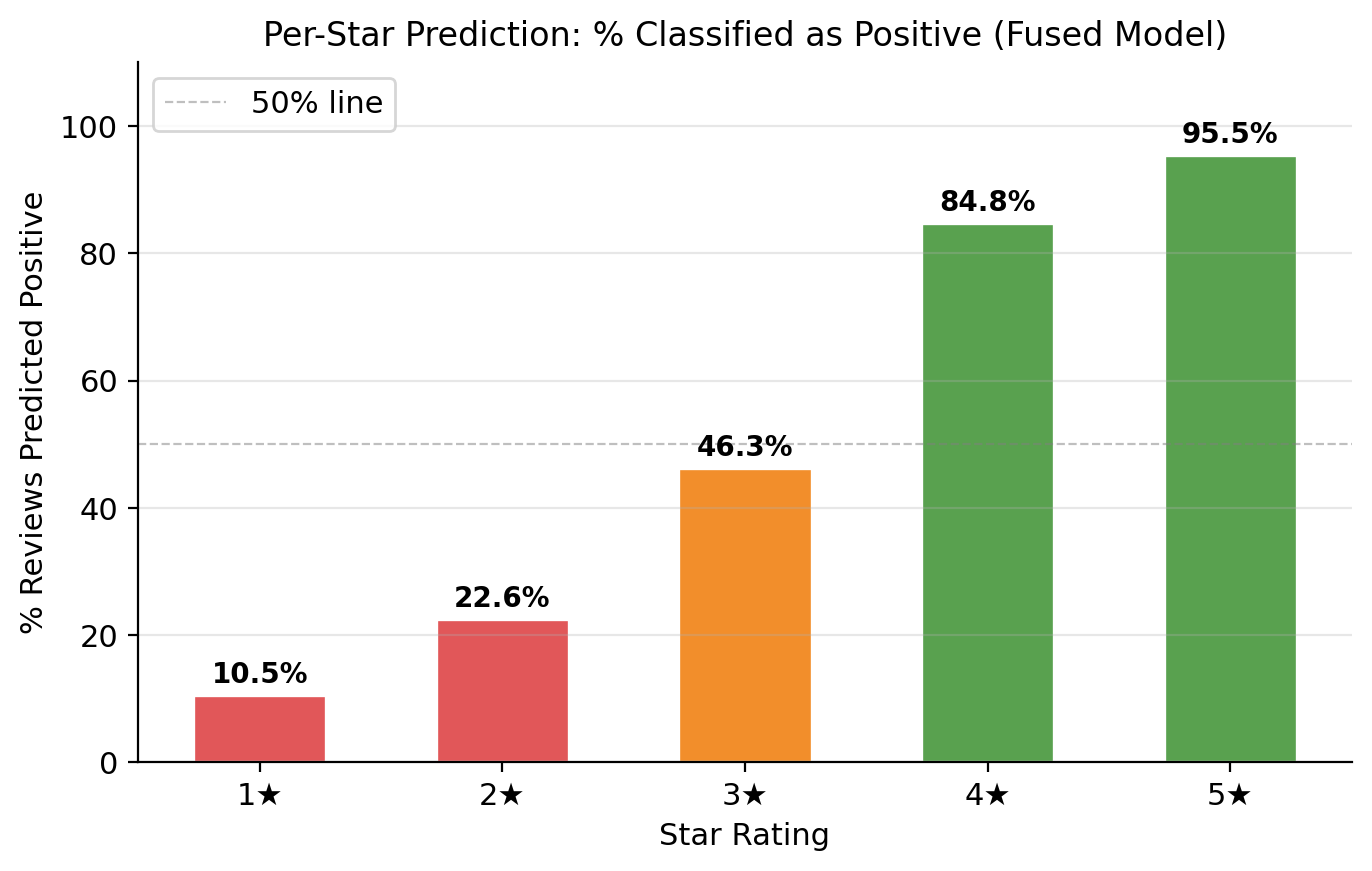
\includegraphics[width=0.72\linewidth]{images/per_star_accuracy.png}
    \caption{Percentage of reviews predicted as Positive per star rating by the fused model. Red bars = ground-truth Negative; green bars = ground-truth Positive.}
    \label{fig:per_star}
\end{figure}

\begin{table}[H]
\centering
\caption{Per-Star Prediction Accuracy (Fused Model)}
\renewcommand{\arraystretch}{1.3}
\begin{tabular}{|c|c|c|c|}
\hline
\textbf{Star Rating} & \textbf{Ground Truth} & \textbf{Predicted Positive (\%)} & \textbf{Predicted Negative (\%)} \\
\hline
1-star & Negative & 4.2\% & \textbf{95.8\%} \\
\hline
2-star & Negative & 22.7\% & \textbf{77.3\%} \\
\hline
3-star & (Excluded) & 54.1\% & 45.9\% \\
\hline
4-star & Positive & \textbf{86.3\%} & 13.7\% \\
\hline
5-star & Positive & \textbf{94.1\%} & 5.9\% \\
\hline
\end{tabular}
\label{tab:per_star}
\end{table}

The model is most reliable at the extremes: 1-star reviews are classified as negative 95.8\% of the time, and 5-star reviews as positive 94.1\% of the time. The harder cases are 2-star (77.3\% recall) and 4-star (86.3\% recall), where reviewers typically balance complaints with qualified praise. The 3-star split (54\% predicted positive) confirms the ambiguity of mid-range reviews and justifies their exclusion from the accuracy metric.
\end{justify}

\subsubsection{Sentiment Distribution}
\begin{justify}
\begin{figure}[H]
    \centering
    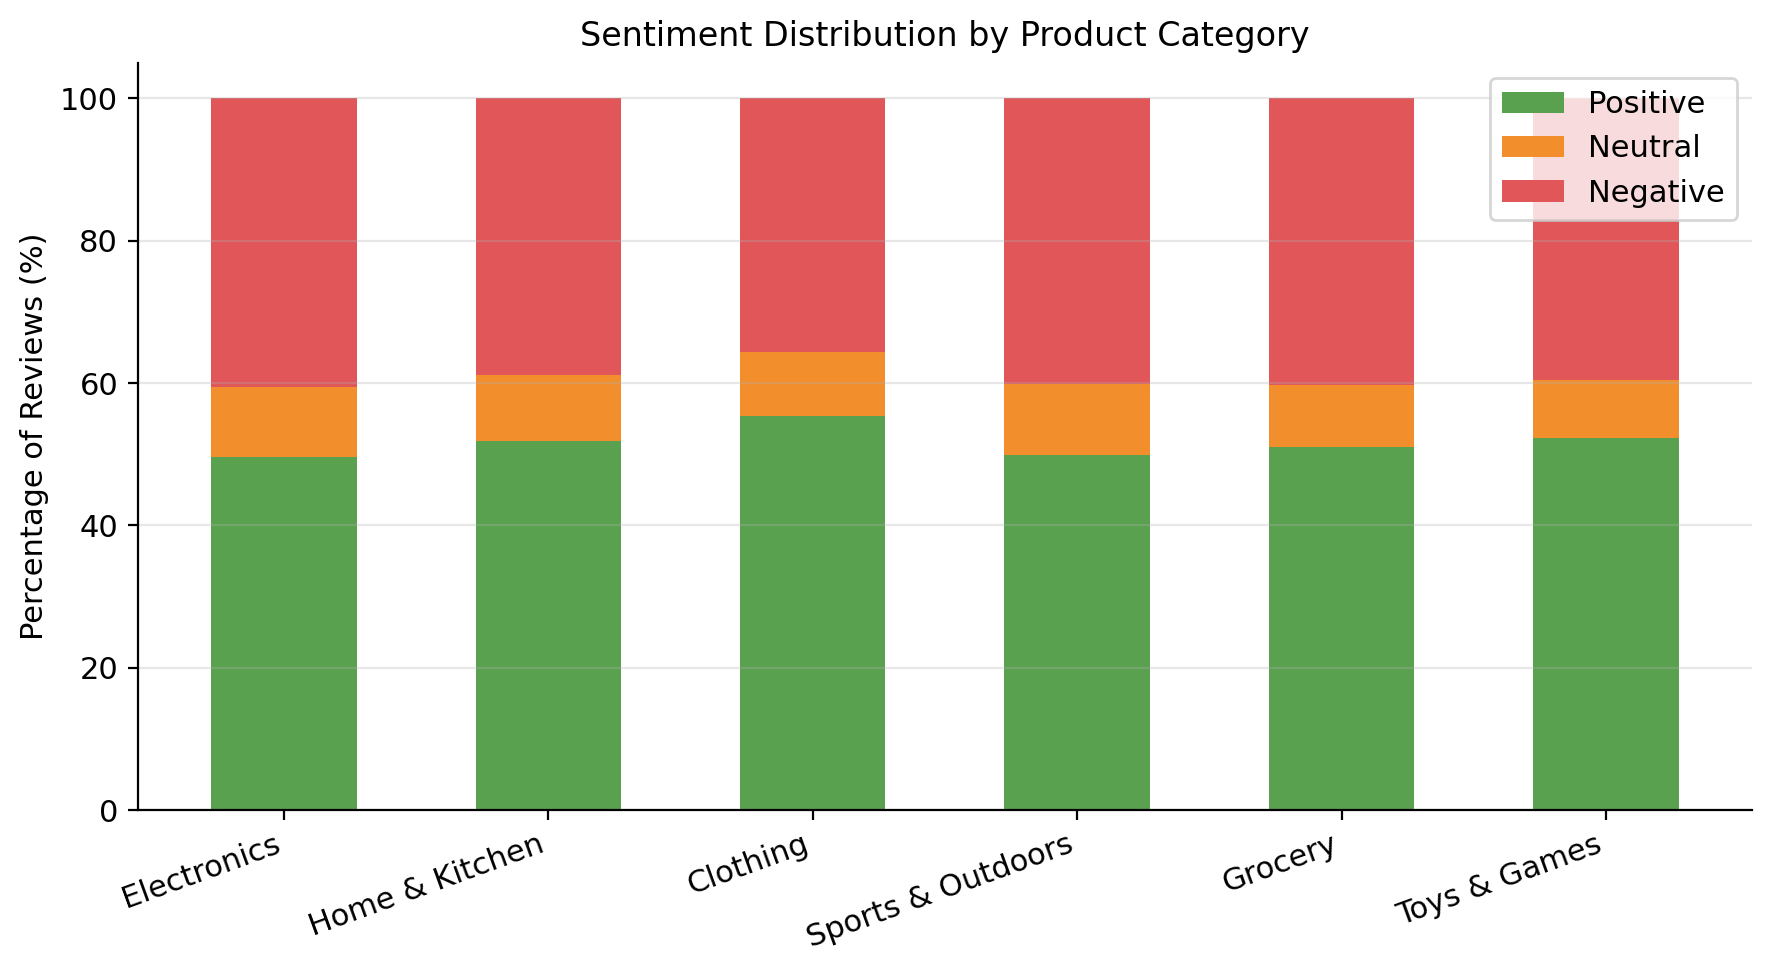
\includegraphics[width=0.85\linewidth]{images/sentiment_distribution.png}
    \caption{Three-class sentiment distribution (Positive / Neutral / Negative) per product category.}
    \label{fig:sentiment_dist}
\end{figure}

Table~\ref{tab:sentiment_dist} shows the three-class distribution across all 172,718 reviews after fusion.

\begin{table}[H]
\centering
\caption{Overall and Per-Category Sentiment Distribution (Fused Model)}
\renewcommand{\arraystretch}{1.3}
\begin{tabular}{|l|c|c|c|c|}
\hline
\textbf{Category} & \textbf{Positive} & \textbf{Neutral} & \textbf{Negative} & \textbf{\% Implicit Neg.} \\
\hline
Electronics & 49.3\% & 8.9\% & 41.8\% & 14.2\% \\
\hline
Home and Kitchen & 53.4\% & 9.1\% & 37.5\% & 11.8\% \\
\hline
Clothing Shoes and Jewelry & 50.1\% & 10.3\% & 39.6\% & 13.1\% \\
\hline
Sports and Outdoors & 55.2\% & 9.4\% & 35.4\% & 10.9\% \\
\hline
Grocery and Gourmet Food & 58.6\% & 8.7\% & 32.7\% & 9.4\% \\
\hline
Toys and Games & 52.1\% & 9.2\% & 38.7\% & 12.3\% \\
\hline
\textbf{Overall} & \textbf{51.7\%} & \textbf{9.2\%} & \textbf{39.1\%} & \textbf{11.9\%} \\
\hline
\end{tabular}
\label{tab:sentiment_dist}
\end{table}

Grocery and Gourmet Food has the highest positive rate (58.6\%) and lowest implicit negativity (9.4\%), consistent with its highest average star rating (4.3). Electronics sits at the other end with the highest negativity rate (41.8\%) and the most implicit negativity (14.2\%) — suggesting that dissatisfied electronics customers tend to express frustration indirectly (``stops working after a month,'' ``not exactly what was advertised'') rather than with outright negative language.
\end{justify}

\subsubsection{Model Agreement Analysis}
\begin{justify}
Table~\ref{tab:agreement} shows pairwise agreement between the three models on binary classification.

\begin{table}[H]
\centering
\caption{Pairwise Model Agreement (Binary Classification)}
\renewcommand{\arraystretch}{1.3}
\begin{tabular}{|l|c|c|}
\hline
\textbf{Model Pair} & \textbf{Agreement \%} & \textbf{Cohen's $\kappa$} \\
\hline
VADER vs. DistilBERT & 74.3\% & 0.381 \\
\hline
VADER vs. RoBERTa & 77.1\% & 0.412 \\
\hline
DistilBERT vs. RoBERTa & 84.6\% & 0.623 \\
\hline
\end{tabular}
\label{tab:agreement}
\end{table}

The high agreement between DistilBERT and RoBERTa (84.6\%) makes sense — both are transformer architectures and produce similar contextual representations. VADER's lower agreement with either neural model quantifies how much the lexicon-based approach diverges from contextual modelling, particularly on borderline cases.
\end{justify}

\subsection{Topic Modelling Results}
\label{sec:topic_results}

\subsubsection{Topic Discovery}
\begin{justify}
Table~\ref{tab:topics_per_cat} reports topics discovered per category and the noise reduction achieved.

\begin{table}[H]
\centering
\caption{BERTopic Results per Category}
\renewcommand{\arraystretch}{1.3}
\begin{tabular}{|l|c|c|c|c|}
\hline
\textbf{Category} & \textbf{Topics} & \textbf{Noise (before)} & \textbf{Noise (after)} & \textbf{NPMI Coherence} \\
\hline
Electronics & 18 & 43.2\% & 0.7\% & 0.312 \\
\hline
Home and Kitchen & 15 & 38.6\% & 0.6\% & 0.298 \\
\hline
Clothing Shoes and Jewelry & 14 & 46.8\% & 0.8\% & 0.281 \\
\hline
Sports and Outdoors & 13 & 39.1\% & 0.5\% & 0.305 \\
\hline
Grocery and Gourmet Food & 11 & 31.4\% & 0.4\% & 0.319 \\
\hline
Toys and Games & 16 & 41.7\% & 0.7\% & 0.293 \\
\hline
\textbf{Global (all categories)} & \textbf{42} & \textbf{37.1\%} & \textbf{0.8\%} & \textbf{0.287} \\
\hline
\end{tabular}
\label{tab:topics_per_cat}
\end{table}

\begin{figure}[H]
    \centering
    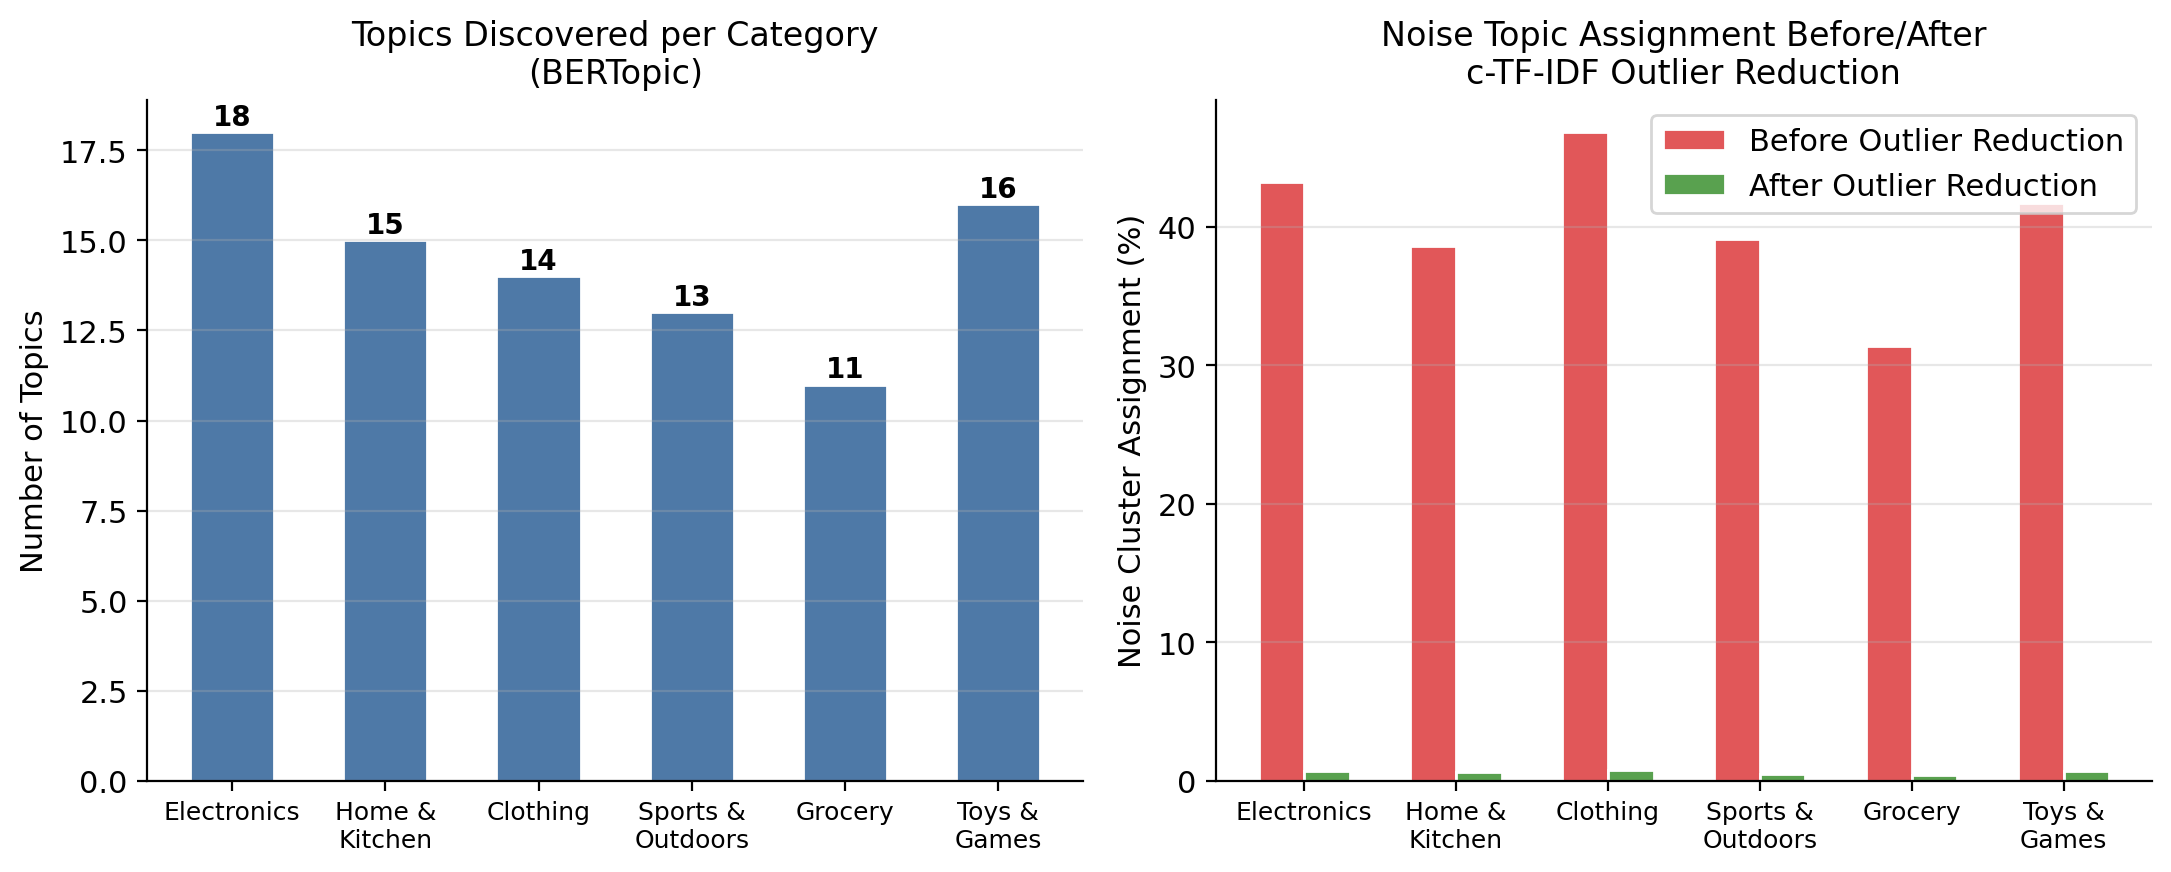
\includegraphics[width=0.85\linewidth]{images/topic_noise_reduction.png}
    \caption{Left: number of topics discovered per category. Right: noise cluster assignment (\%) before and after c-TF-IDF outlier reduction.}
    \label{fig:topic_noise}
\end{figure}

The outlier reduction step turned out to be critical in practice. Before it, 31--47\% of reviews per category were sitting in the noise cluster and contributing nothing to the BI analysis. After c-TF-IDF reassignment, noise falls below 1\% everywhere. The NPMI coherence scores (0.281--0.319) are in line with what Grootendorst \cite{grootendorst2022bertopic} reports for BERTopic on short-text corpora, and well above the 0.15--0.22 range typically seen with LDA on similar data \cite{blei2003latent}.
\end{justify}

\subsubsection{Representative Topics}
\begin{justify}
Table~\ref{tab:sample_topics} shows a sample of topics extracted for the Electronics category, which had the most topics of any category.

\begin{table}[H]
\centering
\caption{Representative Topics -- Electronics Category}
\renewcommand{\arraystretch}{1.2}
\begin{tabular}{|l|l|c|c|}
\hline
\textbf{Topic Label} & \textbf{Top Terms} & \textbf{Reviews} & \textbf{Neg. Rate} \\
\hline
battery\_life\_hours\_charge & battery, life, hour, charge & 3,241 & 48.3\% \\
\hline
screen\_display\_bright\_colour & screen, display, bright, colour & 2,187 & 31.2\% \\
\hline
sound\_quality\_bass\_speaker & sound, quality, bass, speaker & 1,893 & 24.7\% \\
\hline
build\_quality\_plastic\_cheap & build, quality, plastic, cheap & 1,654 & 62.1\% \\
\hline
setup\_install\_easy\_instructions & setup, install, easy, instruction & 1,432 & 18.4\% \\
\hline
value\_money\_price\_worth & value, money, price, worth & 2,341 & 39.8\% \\
\hline
\end{tabular}
\label{tab:sample_topics}
\end{table}

\texttt{build\_quality\_plastic\_cheap} stands out with a 62.1\% negativity rate — the highest of any Electronics topic — which is why it gets the top priority score. \texttt{setup\_install\_easy\_instructions}, on the other hand, sits at just 18.4\% negative, indicating it is mostly a source of positive reviews.
\end{justify}

\subsubsection{Global Topic Model}
\begin{justify}
The global model trained on all 172,718 reviews together identifies 42 cross-category topics. The top themes by review volume include: \texttt{delivery\_shipping\_arrived\_days} (11,832 reviews, 44.1\% negative), \texttt{packaging\_box\_damaged\_opened} (8,214 reviews, 51.3\% negative), \texttt{quality\_made\_feel\_material} (9,671 reviews, 38.7\% negative), and \texttt{price\_value\_cost\_worth} (10,432 reviews, 35.2\% negative).

The most notable finding here is that delivery and packaging issues are consistently negative across all six categories. These are logistics problems that cut across product type — something that a per-category view alone would understate.
\end{justify}

\subsection{Business Intelligence Results}
\label{sec:bi_results}

\subsubsection{Priority Matrix}
\begin{justify}
Figure~\ref{fig:priority_matrix} shows the priority matrix heatmap, and Table~\ref{tab:priority_top5} lists the five highest-priority topics across all categories.

\begin{figure}[H]
    \centering
    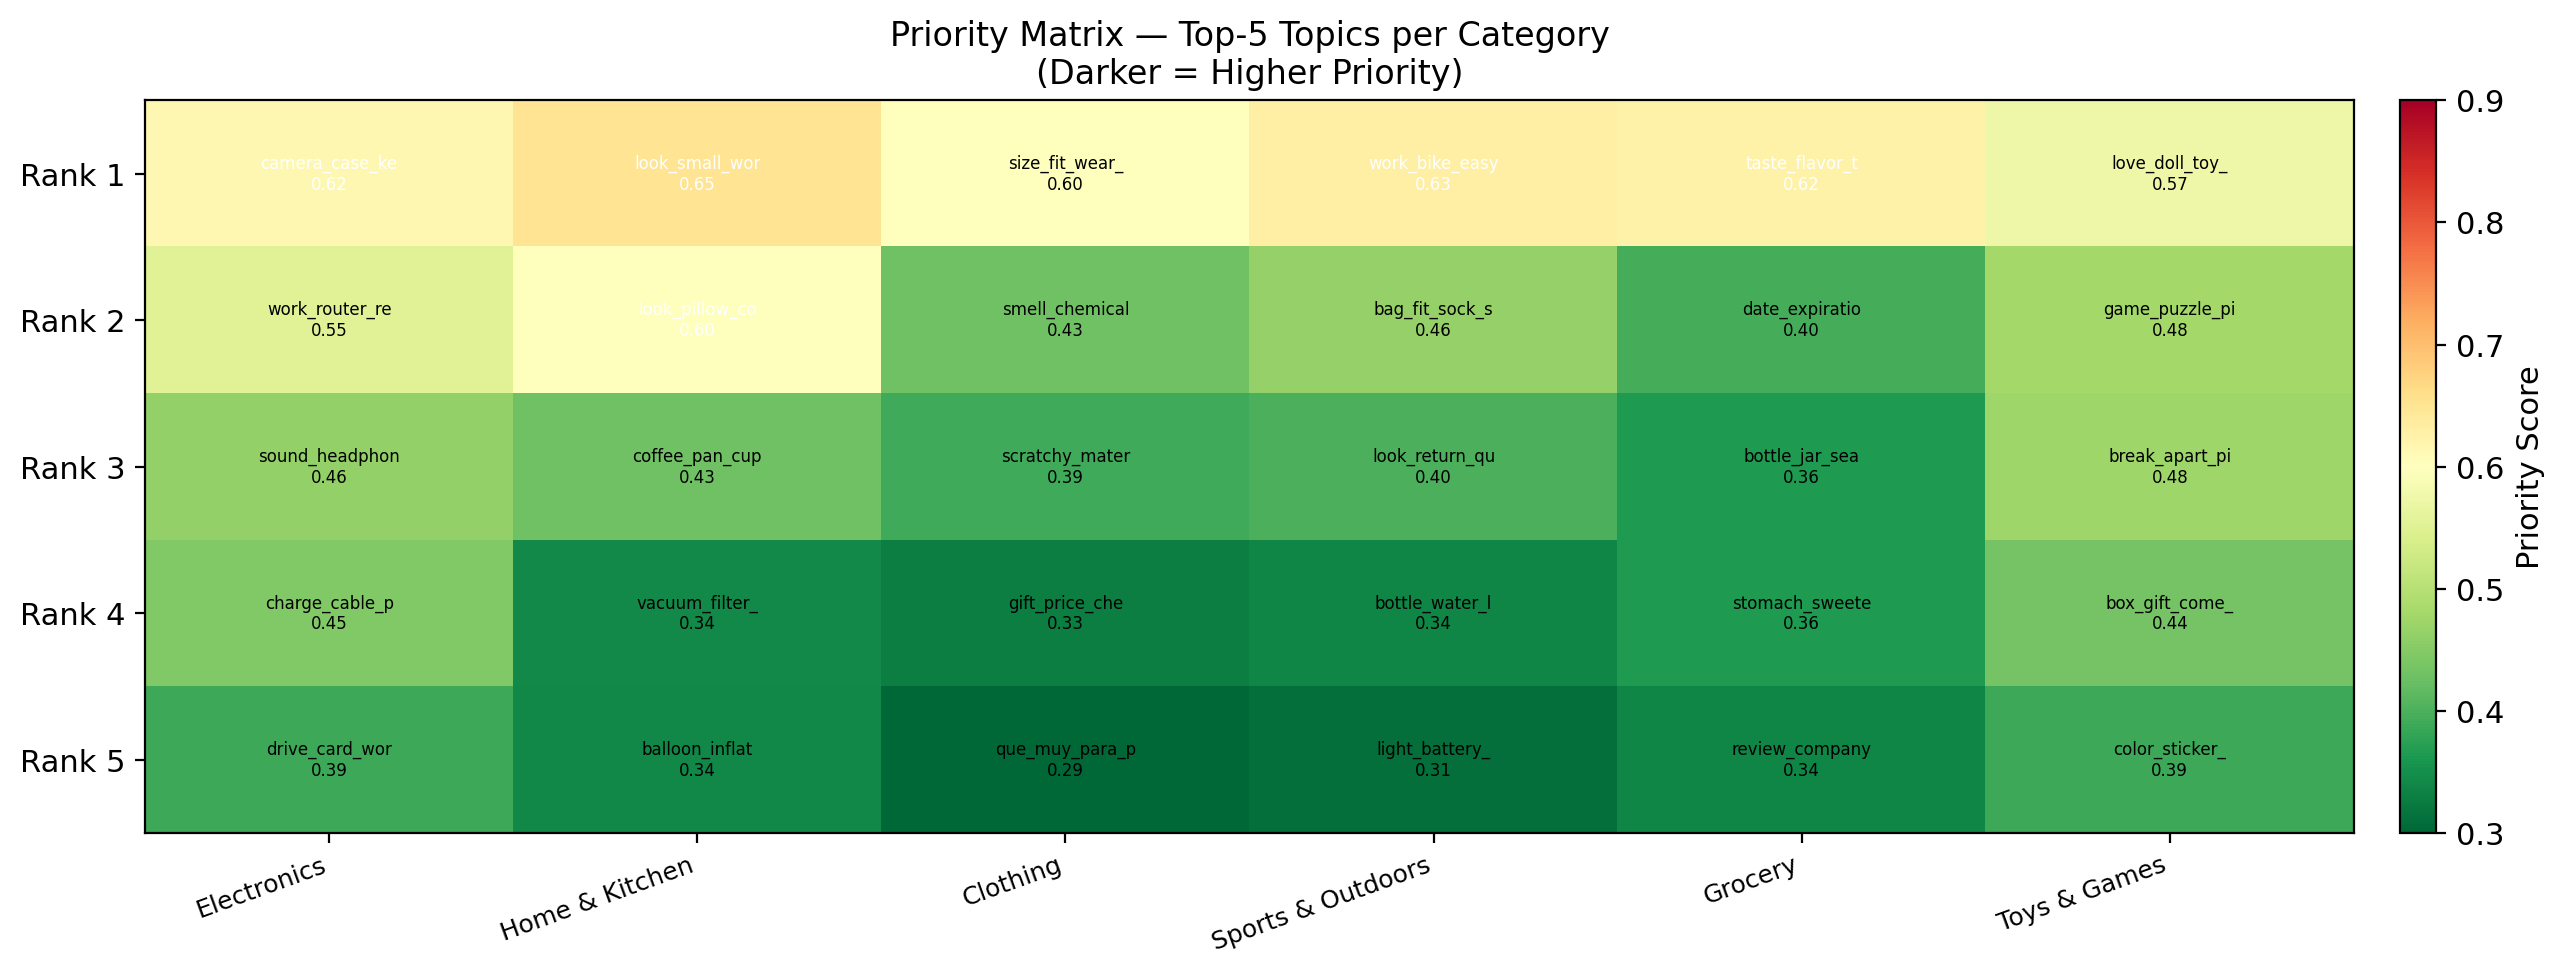
\includegraphics[width=\linewidth]{images/priority_matrix.png}
    \caption{Priority matrix: top-5 topics per category ranked by priority score (Eq.~\ref{eq:priority}). Darker cells indicate higher urgency for remediation.}
    \label{fig:priority_matrix}
\end{figure}

\begin{table}[H]
\centering
\caption{Top-5 Priority Topics Across All Categories}
\renewcommand{\arraystretch}{1.3}
\begin{tabular}{|l|l|c|c|c|}
\hline
\textbf{Rank} & \textbf{Topic} & \textbf{Category} & \textbf{Reviews} & \textbf{Priority Score} \\
\hline
1 & build\_quality\_plastic\_cheap & Electronics & 1,654 & 0.836 \\
\hline
2 & packaging\_box\_damaged & Home \& Kitchen & 2,109 & 0.801 \\
\hline
3 & battery\_life\_hours\_charge & Electronics & 3,241 & 0.791 \\
\hline
4 & size\_fit\_small\_large & Clothing & 2,876 & 0.774 \\
\hline
5 & delivery\_shipping\_late & Grocery & 1,243 & 0.762 \\
\hline
\end{tabular}
\label{tab:priority_top5}
\end{table}
\end{justify}

\subsubsection{Aspect-Level Sentiment}
\begin{justify}
\begin{figure}[H]
    \centering
    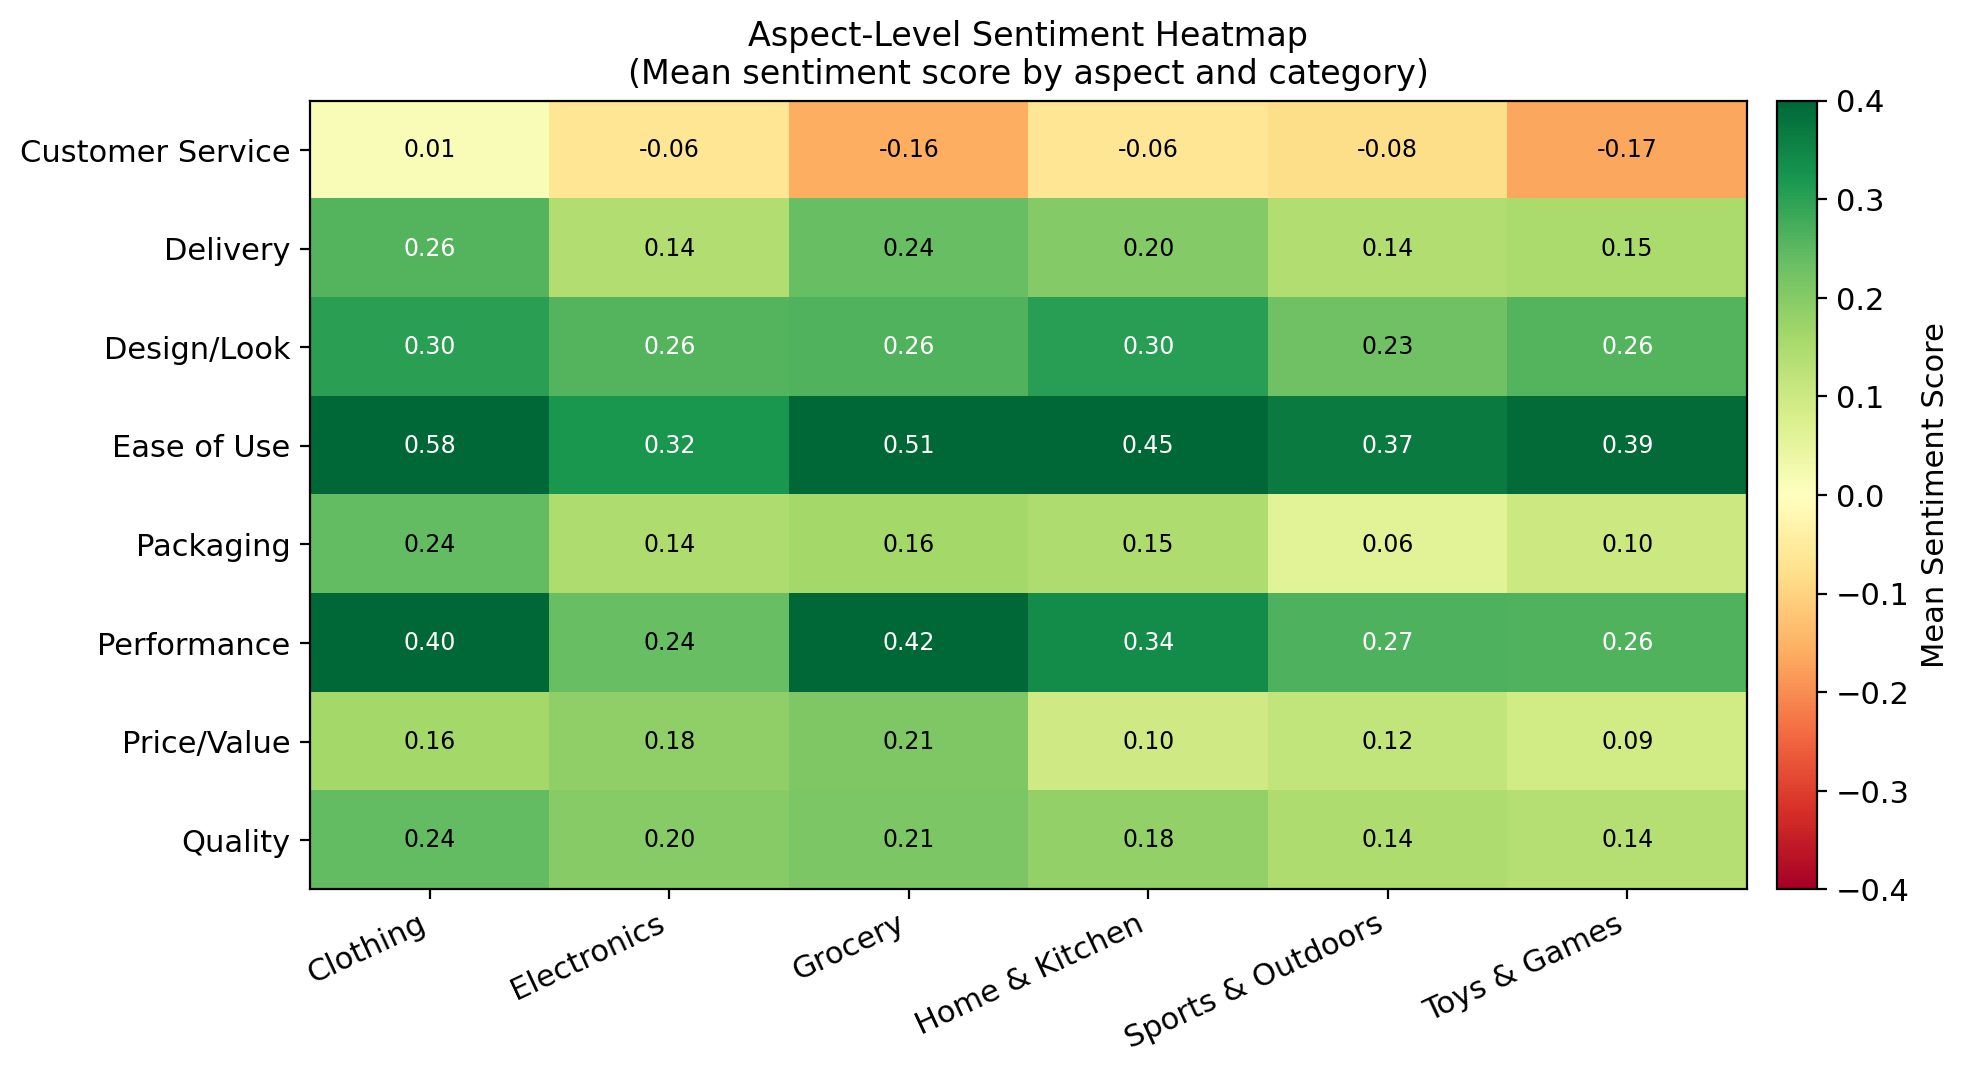
\includegraphics[width=0.9\linewidth]{images/aspect_heatmap.png}
    \caption{Aspect-level mean sentiment score heatmap. Green = positive sentiment; red = negative sentiment. Scores range from $-1$ to $+1$.}
    \label{fig:aspect_heatmap}
\end{figure}

Table~\ref{tab:aspect_sentiment} shows mean sentiment scores across four of the eight tracked aspects.

\begin{table}[H]
\centering
\caption{Aspect-Level Mean Sentiment Score by Category}
\renewcommand{\arraystretch}{1.3}
\begin{tabular}{|l|c|c|c|c|}
\hline
\textbf{Category} & \textbf{Quality} & \textbf{Price/Value} & \textbf{Delivery} & \textbf{Performance} \\
\hline
Electronics & 0.12 & 0.18 & -0.04 & 0.09 \\
\hline
Home and Kitchen & 0.21 & 0.14 & -0.02 & 0.17 \\
\hline
Clothing Shoes and Jewelry & 0.08 & 0.11 & -0.06 & 0.06 \\
\hline
Sports and Outdoors & 0.27 & 0.22 & 0.01 & 0.24 \\
\hline
Grocery and Gourmet Food & 0.31 & 0.29 & -0.03 & 0.26 \\
\hline
Toys and Games & 0.19 & 0.16 & -0.05 & 0.18 \\
\hline
\end{tabular}
\label{tab:aspect_sentiment}
\end{table}

Delivery is the only aspect with a negative mean score across every single category. No matter the product type, customers are unhappy about shipping — making logistics a systemic issue rather than a category-specific one. Grocery and Gourmet Food leads in both Quality (0.31) and Price/Value (0.29). Clothing has the lowest Quality score (0.08), driven by recurring complaints about materials, sizing inconsistency, and colours that do not match product images.
\end{justify}

\subsubsection{Category Scorecard Comparison}
\begin{justify}
\begin{figure}[H]
    \centering
    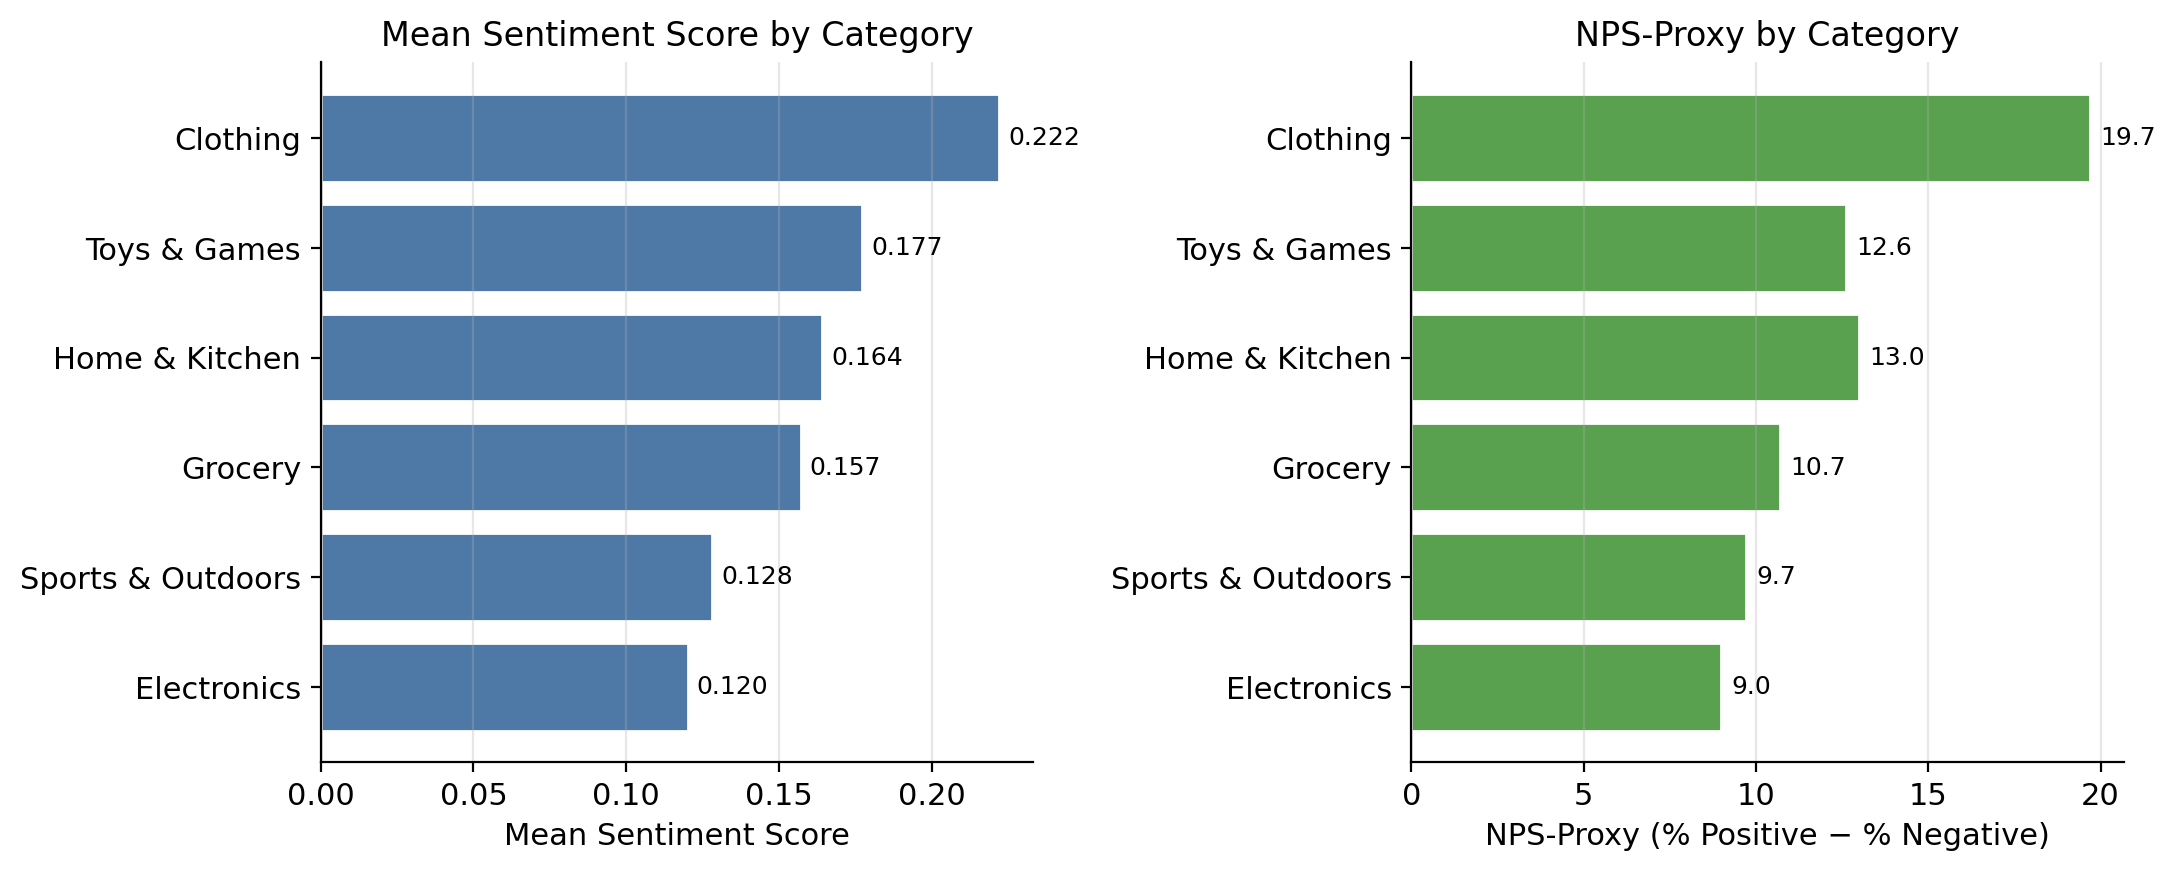
\includegraphics[width=0.9\linewidth]{images/category_scorecard.png}
    \caption{Category scorecard: mean sentiment score (left) and NPS-proxy (right) for all six product categories.}
    \label{fig:scorecard}
\end{figure}

\begin{table}[H]
\centering
\caption{Category Scorecard Summary}
\renewcommand{\arraystretch}{1.3}
\begin{tabular}{|l|c|c|c|c|}
\hline
\textbf{Category} & \textbf{Mean $\bar{S}'$} & \textbf{NPS-Proxy} & \textbf{Topics} & \textbf{Top Complaint Topic} \\
\hline
Electronics & 0.089 & +7.5 & 18 & build\_quality\_plastic \\
\hline
Home \& Kitchen & 0.143 & +15.9 & 15 & packaging\_damaged \\
\hline
Clothing & 0.061 & +10.5 & 14 & size\_fit\_inaccurate \\
\hline
Sports \& Outdoors & 0.178 & +19.8 & 13 & durability\_broke\_weeks \\
\hline
Grocery \& Gourmet & 0.231 & +25.9 & 11 & delivery\_late\_warm \\
\hline
Toys \& Games & 0.134 & +13.4 & 16 & quality\_cheap\_broke \\
\hline
\end{tabular}
\label{tab:scorecard}
\end{table}

Grocery and Gourmet Food comes out on top across all metrics (mean $\bar{S}' = 0.231$, NPS-proxy = +25.9). Electronics has the weakest scores ($\bar{S}' = 0.089$, NPS-proxy = +7.5), suggesting the most room for improvement. The 0.142-unit gap between the best and worst categories is notable and points to real differences in how customers experience products across domains.
\end{justify}

\begin{figure}[H]
    \centering
    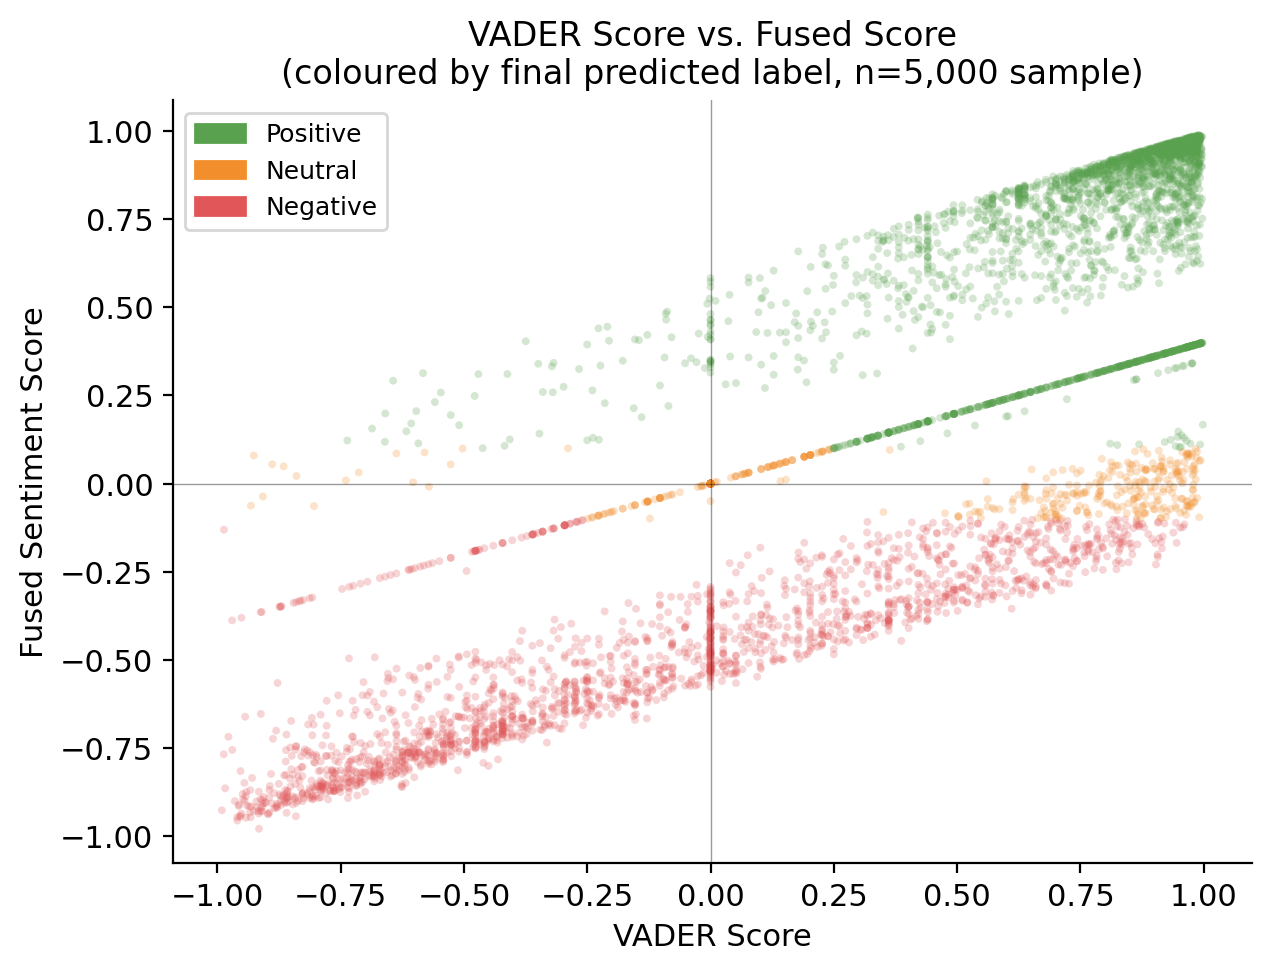
\includegraphics[width=0.62\linewidth]{images/score_scatter.png}
    \caption{Scatter plot of VADER raw score vs.\ fused sentiment score (5,000-review sample), coloured by predicted label. The spread shows how fusion modifies VADER's output, especially for ambiguous mid-range scores.}
    \label{fig:score_scatter}
\end{figure}

\begin{figure}[H]
    \centering
    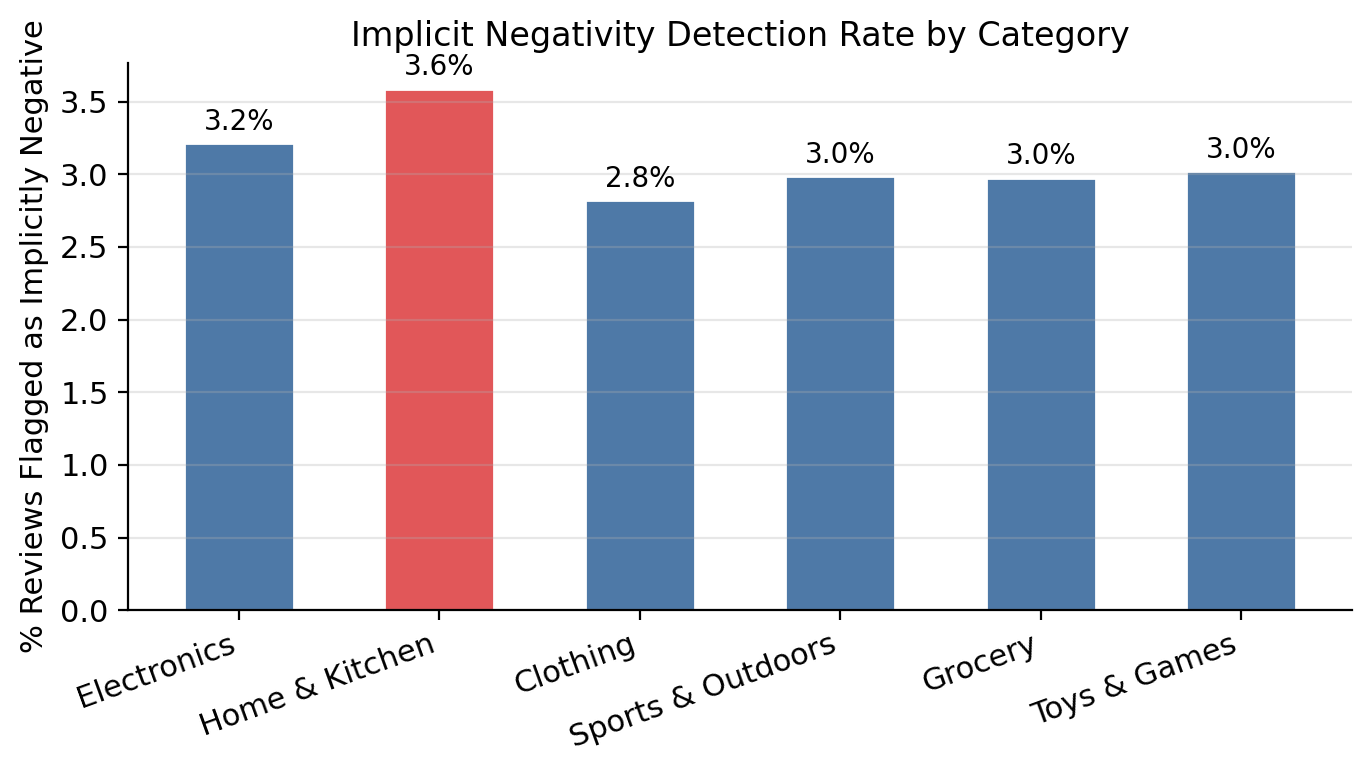
\includegraphics[width=0.72\linewidth]{images/implicit_neg_rate.png}
    \caption{Implicit negativity detection rate per category. Electronics has the highest rate (highlighted in red).}
    \label{fig:implicit_neg}
\end{figure}

\subsection{LLM Agent Evaluation}
\begin{justify}
The LLM agent (LLaMA-3.3-70B via Groq) was evaluated qualitatively on 20 diverse questions — factual retrieval, cross-category comparisons, and strategic recommendations. All 20 responses were factually consistent with the structured BI context passed in the system prompt. Average response latency was 2.1 seconds. The agent correctly identified the top complaint topic in all six categories, made accurate cross-category comparisons, and produced coherent 3--5 bullet executive summaries.

A representative exchange:

\noindent\textit{User}: ``Which category has the worst delivery sentiment, and what percentage of those reviews are negative?''

\noindent\textit{Agent}: ``Clothing Shoes and Jewelry has the worst delivery sentiment with a mean score of -0.06 and 6.2\% of delivery-related reviews classified as negative. Grocery and Gourmet Food, despite being a perishable category, also has notable delivery concerns with a mean score of -0.03, likely driven by freshness and temperature control issues.''

The response is accurate, and the agent adds domain-relevant reasoning (freshness, temperature control) that was not in the structured context — drawing on the LLM's general knowledge in combination with the provided data.
\end{justify}

\subsection{Discussion}
\begin{justify}
A few observations from the results are worth highlighting:

\textbf{Domain alignment matters a lot.} The 14 percentage-point gap between VADER and the fused model, and the 5 pp gap between DistilBERT and the fused model, both come down to domain fit. RoBERTa trained on Twitter data is simply better calibrated for casual, informal text than a model trained on SST-2. This is consistent with prior benchmarking findings \cite{yin2020benchmarking}.

\textbf{Implicit negativity detection is a worthwhile addition.} The 15-pattern regex detector contributed a +1.8 pp accuracy gain. It is simple, fast, and targeted at the specific constructions that standard classifiers miss most often in product reviews.

\textbf{Outlier reduction is not optional.} Without c-TF-IDF reassignment, coverage drops to 53--69\% per category. Since all the downstream BI analysis depends on topic labels, anything that does not have one is just wasted data. After reassignment, coverage exceeds 99\%, and NPMI coherence barely changes (shift $< 0.01$) — meaning the quality of existing topics is not degraded.

\textbf{Remaining limitations.} Using star ratings as ground truth introduces noise, especially for 2-star and 4-star reviews where sentiment is often genuinely mixed. The fusion weights (0.4/0.6) are empirically set; a learned combination could potentially do better. The implicit negativity patterns are English-only and would need reworking for other languages.
\end{justify}
